\documentclass{article}
\usepackage[utf8]{inputenc}
\usepackage{url}
\title{A Grocery Placing Robot for in Home Assistance}
\author{Zhenkai Gao, Alex Kautz, Pascale Leone}
\date{\vspace{-1em}}

\usepackage{natbib}
\usepackage{graphicx}
\usepackage{caption}
\usepackage{float}
\usepackage{xurl}

\begin{document}

\maketitle

% for final report only
%\begin{abstract}
%A one paragraph high level description of the work. The abstract is typically the first thing someone would read from the paper before deciding whether to continue reading and hence, serves as an advertisement to the reader to read the whole paper. 
%\end{abstract}

\section{Introduction}


Imagine a future where you receive a box of groceries from a delivery service (like Amazon), you take the box to your kitchen table and open it. Then your helpful robot arm takes items out of the box and places them in your refrigerator in their best position.

This project is to program a robotic arm (in a simulation) to help a person unpack their grocery delivery order. Our robot should classify grocery items as frozen, refrigerated, or non-perishable. This system could be used to assist the elderly or disabled. It could also easily be extended to help with inventory management in professional kitchens or grocery stores.


\section{Background Related Work}

Assisting the elderly with household tasks is a common application for robotics. In 1998, a team based out of Italy developed MOVAID. The MOVAID system consisted of a robotic arm attached to a driving base. MOVAID's goal was to assist in 3 main tasks: heating up food, cleaning the kitchen, and changing bed sheets. As part of that first task, the robot had to take food out of the refrigerator \cite{doi:10.3233/TAD-1999-10202}.


Similar to this work, we want to use a robotic arm to unpack and place groceries. We believe this task is important because it can help the elderly or disabled in the kitchen. We will use a static robot arm rather than a moving base and focus on the task of putting away groceries. This task involves three key areas: object detection, trajectory planning, and stable placement.

Object detection in a cluttered environment is an important problem. Researchers at Jaume I University in Castellon de la Plana, Spain studied object detection in a cluttered scene in order to help the BAXTER robot pick the correct object in a cluttered environment \cite{10.1145/3164541.3164628}. They employed deep learning methods to improve performance, and ultimately found that RESNET, a semantic segmentation based method, for object detection produced more accurate results than a localization method with YOLO. 

Trajectory planning is also relevant to our problem. Our robotic arm must navigate from the box of groceries to the appropriate storage container, without hitting any obstacles. Researchers in the Department of Mechatronics Engineering at the Isparta University of Applied Sciences in Isparta Turkey studied trajectory planning for a robotic arm with 6 degrees of freedom \cite{EKREM2023106099}. Their experiments focused on the Particle Swarm Optimization (PSO) algorithm, which is a population-based stochastic optimization method. This algorithm starts with a population of random solutions and searches for the optimal solution by updating generations. They proposed that the PSO algorithm optimizes trajectory planning of the 6-degree-of-freedom. 
\begin{figure}[H]
    \centering
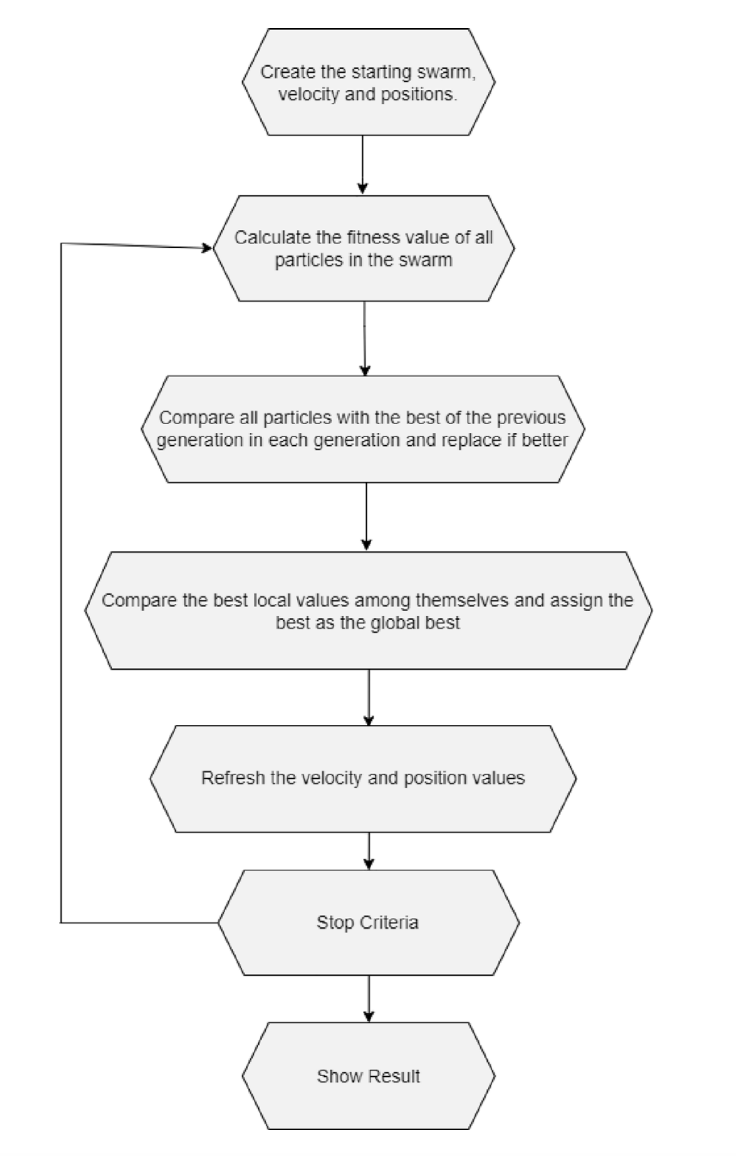
\includegraphics[width=0.5\linewidth]{PSO.png}
    \caption*{PSO Algorithm Flow Chart \cite{EKREM2023106099}}
    \label{fig:placeholder}
\end{figure}
It is also important that our robot is able to facilitate stable placement of each grocery item. As the storage containers accumulate objects, the robot must determine an appropriate location for the new grocery item. Haustein, Hang, Stork, and Kragic address the problem of placement planning by creating an algorithm that computes placements for objects based on three main principles: (1) suitable locations must be identified, (2) placements must be reachable, and (3) not all placements are equally desirable \cite{8967732}.
\begin{figure}[H]
    \centering
    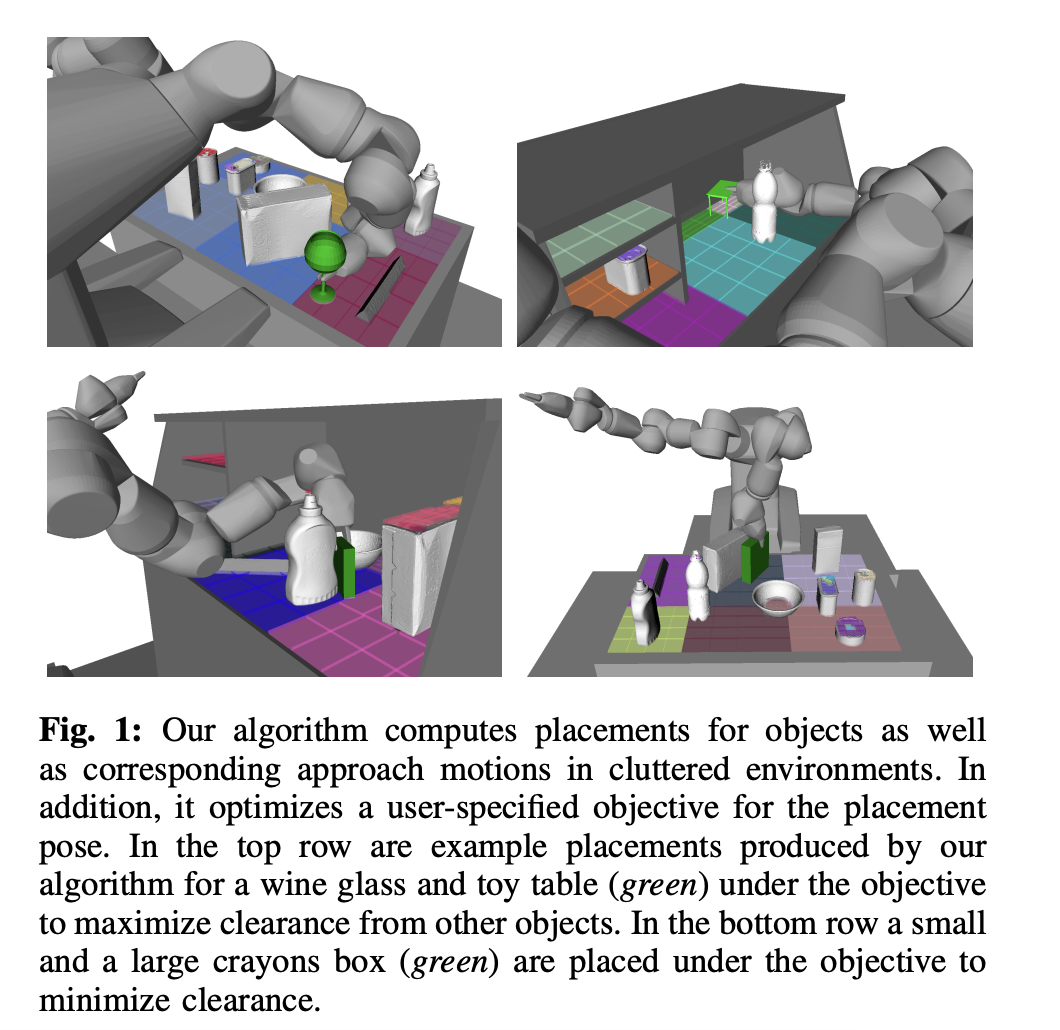
\includegraphics[width=0.65\linewidth]{placements.png}
    \caption*{Example optimized placements \cite{8967732}}
    \label{fig:placeholder}
\end{figure}

\section{Technical Approach / Methodology / Theoretical Framework}

% for proposal


% Alex: not sure if we need this part anymore
% To approach this problem we will break it down into three core areas and tackle them separate separately before combining. The core areas are:
% \begin{itemize}
% \item Using computer vision to identify and locate objects within a crowded box.
% \item Using a formal logic to identify where each object in the box goes in the refrigerator, keeping in mind existing objects in the refrigerator.
% \item Using inverse kinematics to actually move the robotic arm to manipulate the objects.
% \end{itemize}

\subsection{Simulation}
We will use the Gazebo robot simulator \url{https://gazebosim.org/home} \cite{1389727}. 
\begin{itemize}
    \item We adopt the Kinova Gen 3 robotics arm as the robot manipulator integrated into our simulation environment.
    \item Simulating a Kinova Gen 3 robotic arm \newline \url{https://www.kinovarobotics.com/product/gen3-robots/}
   
    by following the MoveIt2 tutorial 
    \newline
    \url{https://moveit.picknik.ai/main/doc/tutorials/quickstart_in_rviz/quickstart_in_rviz_tutorial.html}
   
    based on the real-life model by Kinova Robotics for motion planning.
    
    \item Simulating a camera attached to the robotic arm.
    \item Creating a virtual environment consisting of:
    \begin{itemize}
        \item The robot and camera themselves.
        \item A fixed box with an open top.
        \item A selection of grocery items (e.g., an apple, a cereal box, etc.) sitting in the box.
        \item A shelf, representing an open refrigerator.
    \end{itemize}
\end{itemize}

\subsection{Vision}
For the vision component of our project, we will use a two-part pipeline.

First, we use the YOLO (You Only Look Once) network to identify which grocery items are in the box and their approximate locations within it \cite{DBLP:journals/corr/RedmonDGF15}. This is aided by a preexisting database of grocery items that may appear in the box.

We then use ResNet \cite{10.1145/3164541.3164628} to segment the image. ResNet produces a mask surrounding the edge of each object. We can then use this to estimate the object's location in 3D space, allowing the arm to grasp it.

We will also use 3D camera to gain better location information for each object.

\subsection{Logic}

After a grocery item has been identified, it is classified into one of three groups using an existing mapping of grocery items to groupings.

The groups are frozen, refrigerated, and non-perishable. Each group corresponds to a shelf on the refrigerator. The robot tracks how much space remains on each shelf so that it knows where to place each item. If there is no more space on a shelf for a given item, the system sends an alert.

% for final report
%A detailed description of your problem (with math, notation, algorithms, figures, etc.). Use footnotes to cite links to your code or videos\footnote{All developed source code for this project is available at ...}

\subsection{Tasks}


The tasks for this project cover the individual parts ranging from simplified versions to more complex versions.


Computer Vision
\begin{itemize}
    \item identify a single grocery object.
    \item identify a single grocery object and its location.
    \item identify multiple grocery objects and their locations when they are spread apart.
    \begin{sloppypar}
    \item identify multiple grocery objects and their locations when they are grouped closely together.
    \end{sloppypar}
    \item identify multiple grocery objects and their locations when they overlap (by being placed on top of one another).
\end{itemize}

Formal Planning
\begin{itemize}
    \item for single grocery object, identify appropriate refrigerator section.
    \item determine (optimal) path from grocery box to refrigerator section.
    \item determine stable placement of grocery item in storage section, based on existing items.
\end{itemize}

Manipulation and Simulation Environment Setup
\begin{itemize}
    \item Inverse Kinematics: determine joint positions required for grasping and placing an object, given the object's coordinate in the global map frame.
    \item Gazebo Environment architecture: design the high-fidelity simulation environment, including the UR3 URDF integration, grocery container models, and target fridge.
    \item MoveIt 2 Configuration: set up the motion planning framework. This includes defining the UR3’s Planning Groups, and configuring OMPL planners for low-level planning to generate a collision-free trajectory. 
    \item Collision Avoidance: implement a real-time Octomap server that consumes the wrist-camera’s point cloud. The system will be configured to dynamically update the planning scene so the UR3 avoids hitting the edges of the box or other groceries during its movement.
    \item Gripper Control: implement the hardware interface for a simulated gripper. This provides high-level services for grasp and release commands.
\end{itemize}

% for final report
%\section{Experimental Results / Technical Demonstration}

%A description of how you evaluated or demonstrated your solution.\footnote{a video of the robot doing x y z is available at...} 

% for proposal
\section{Evaluation}

We evaluate our system at multiple levels of granularity, measuring both end-to-end performance and the effectiveness of individual subsystems.

\subsection*{Metrics}
\begin{description}
    \item[Overall success rate:] The percentage of grocery items successfully placed during a full run, averaged over multiple trials.
    \item[Computer vision accuracy:] The percentage of objects correctly identified from the input image.
    \item[Manipulation reliability:] Given accurate object identification and a specified destination, the percentage of successful pick-and-place operations without dropping the object.
    \item[Planning quality:] Whether the arm collides with surrounding objects (e.g., the kitchen table) during pick-and-place, and the time elapsed per operation.
\end{description}

\subsection*{Experimental Variations}
We compare these metrics under the following conditions:

\paragraph{Grocery density.}
We vary how closely items are placed in the box, following our staged task plan for computer vision:
\begin{enumerate}
    \item A single item in the box.
    \item Multiple items spread apart.
    \item Multiple items clustered together.
    \item Multiple items overlapping.
\end{enumerate}

\paragraph{Camera configuration.}
We plan to use both a 2D camera (YOLO and ResNet) and a 3D camera for grocery item localization. As a variation, we evaluate performance using only the 2D camera.

\paragraph{Item shape and size.}
We track which grocery item geometries yield the best manipulation and transfer performance. A formal experiment can be run if the initial results appear significant.

% for final report
%\section{Conclusion and Future Work}

%A high level summary of what was accomplished, along with a discussion on limitations and avenues for future work (typically 2 to 3 paragraphs). 


\section{Timeline and Individual Responsibilities}
\noindent Weeks 1-2:
\begin{enumerate}
    \item Set up Gazebo simulation environment.
    \item Create mapping of grocery items to storage location.
    \item Set up computer vision model.
\end{enumerate}
Weeks 3-4:
\begin{enumerate}
    \item Determine optimal path plan.
    \item Determine stable placement plan.
\end{enumerate}
Weeks 5-6:
\begin{enumerate}
    \item Test and make final changes to program.
    \item Evaluate success under varied conditions based on defined metrics.
    \item Generate figures and write final report.
\end{enumerate}

\noindent Generally, Alex will focus on computer vision tasks, Zhenkai will focus of robot manipulation tasks, and Pascale will focus on planning tasks. There is significant overlap between the three divisions, so we will work together as needed, particularly in the project setup phase. In addition, final testing and report generation will be done by everyone.
%\cite{short2010no}.

\bibliographystyle{plain}
\bibliography{references}
\end{document}
